%%%%%%%%%%%%%%%%%%%%%%%%%%%%%%%%%%%%%%%%%%%%%%%%%%%%%%%%%%%%%%%%%%%
%TO AVOID FORMATTING ISSUES, COMPILE THIS ONLY AT WWW.OVERLEAF.COM%
%%%%%%%%%%%%%%%%%%%%%%%%%%%%%%%%%%%%%%%%%%%%%%%%%%%%%%%%%%%%%%%%%%%
%%%%%%%%%%%%%%%%%%%%%%%%%%%%%%%%%%%%%%%%%%%%%%%%%%%%%%%%%%%%%%%%%%%
\documentclass[a4paper,12pt]{article}
\usepackage[ascii]{inputenc}
\usepackage{amsmath}
\usepackage{amssymb,amsfonts,textcomp}
\usepackage[T1]{fontenc}
\usepackage[english]{babel}
\usepackage{color}
\usepackage{array}
\usepackage{supertabular}
\usepackage{hhline}
\usepackage{hyperref}
\hypersetup{pdftex, colorlinks=true, linkcolor=blue, citecolor=blue, filecolor=blue, urlcolor=blue, pdftitle=, pdfauthor=KDvenu, pdfsubject=, pdfkeywords=}
\usepackage[pdftex]{graphicx}
% Outline numbering
\setcounter{secnumdepth}{0}
\makeatletter
\newcommand\arraybslash{\let\\\@arraycr}
\makeatother
% Page layout (geometry)
\setlength\voffset{-1in}
\setlength\hoffset{-1in}
\setlength\topmargin{0.5in}
\setlength\oddsidemargin{0.8916in}
\setlength\textheight{10.274333in}
\setlength\textwidth{5.9847994in}
\setlength\footskip{12.0pt}
\setlength\headheight{0.252in}
\setlength\headsep{0cm}
% Footnote rule
\setlength{\skip\footins}{1.1777999mm}
\renewcommand\footnoterule{\vspace*{-0.007in}\setlength\leftskip{0pt}\setlength\rightskip{0pt plus 1fil}\noindent\textcolor{black}{\rule{0.33\columnwidth}{0.007in}}\vspace*{1mm}}
% Pages styles
\makeatletter
\newcommand\ps@MP{
  \renewcommand\@oddhead{}
  \renewcommand\@evenhead{\@oddhead}
  \renewcommand\@oddfoot{}
  \renewcommand\@evenfoot{\@oddfoot}
  \renewcommand\thepage{\arabic{page}}
}
\makeatother
\pagestyle{MP}
\setlength\tabcolsep{1mm}
\renewcommand\arraystretch{1.3}
\title{}
\author{}
\date{21-03-2016}
\usepackage{graphicx}
%To use this font, you need XeTex or LuaTex, prefer openleaf
\newenvironment{codeblock}{\fontfamily{ccr}\selectfont}{\par}

\title{
	\normalfont \normalsize 
	\textsc{Pimpri Chinchwad College of Engineering \\ 
		Computer Laboratory - IV} \\
	[10pt]   
	\rule{\linewidth}{0.5pt} \\[6pt] 
	\huge Assignment No - B6 \\
	\rule{\linewidth}{2pt}  \\[10pt]
}
\author{}
\date{\normalsize}


\begin{document}
	\maketitle
\setcounter{page}{1}\pagestyle{MP}

\bigskip

{\sffamily
\textrm{\textbf{AIM:\ {}-}}\textrm{\ 8-Queens Matrix is Stored using JSON/XML having first Queen placed, use back-tracking to place
remaining Queens to generate final 8-queen's Matrix. Use suitable Software modeling , Design and
testing methods. Justify the selection over other methods.}}


\bigskip

{\sffamily
\textrm{\textbf{THEORY:}}}

{\ttfamily
\textrm{The\ }\textrm{\textbf{Eight queens puzzle}}\textrm{\ is the problem of placing
eight\ }\href{https://en.wikipedia.org/wiki/Chess}{\textrm{\textcolor[rgb]{0.0,0.0,0.5019608}{chess}}}\textrm{\ }\href{https://en.wikipedia.org/wiki/Queen_\%28chess\%29}{\textrm{\textcolor[rgb]{0.0,0.0,0.5019608}{queens}}}\textrm{\ on an 8{\texttimes}8 chessboard so that no two queens threaten each other. Thus, a solution requires that no two queens share the same row, column, or diagonal. The eight queens puzzle is an example of the more general\ }\textrm{\textbf{\textit{n}}}\textrm{\textbf{{}-queens problem}}\textrm{\ of placing\ }\textrm{\textit{n}}\textrm{\ queens on an\ }\textrm{\textit{n}}\textrm{{\texttimes}}\textrm{\textit{n}}\textrm{\ chessboard, where solutions exist for all natural numbers\ }\textrm{\textit{n}}\textrm{\ with the exception of\ }\textrm{\textit{n}}\textrm{=2 and\ }\textrm{\textit{n}}\textrm{=3.}}

{\color{black}
For example:\ }

{\color{black}
\ \ \ \ \ Q1 attacks some positions, therefore Q2 has to comply with these constraints and take its place, not directly
attacked by Q1. Placing Q3 is harder, since we have to satisfy constraints of Q1 and Q2. Going the same way we may reach
point, where the constraints make the placement of the next queen impossible. Therefore we need to relax the
constraints and find new solution.}

{\color{black}
\ \ \ \ \ To do this we are going backwards and finding new admissible solution. To keep everything in order we keep the
simple rule: last placed, first displaced. In other words if we place successfully queen on the ith column but cannot
find solution for (i+1)th queen, then going backwards we will try to find other admissible solution for the ith queen
first. This process is called backtracking.}


\bigskip

 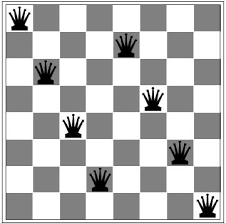
\includegraphics[width=5.60417in,height=4.14583in]{queen-img001.png} 

\clearpage
\bigskip

\noindent \textbf{UML diagrams :}\\
\begin{itemize}
\item \textbf{Class diagram :}
\begin{figure}[h!]
		\centering
		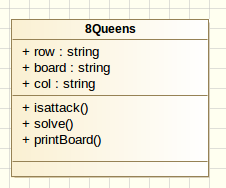
\includegraphics[scale=0.5]{class_diagram.png}
	\end{figure}
\item \textbf{Sequence diagram :}
\begin{figure}[h!]
		\centering
		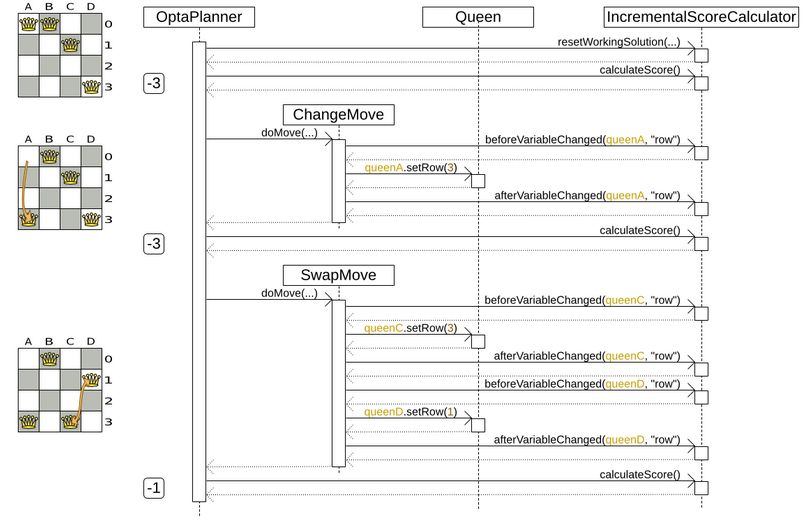
\includegraphics[scale=0.5]{Seq8queens.png}
	\end{figure}
	
\item \textbf{Activity diagram :}
\begin{figure}[h!]
		\centering
		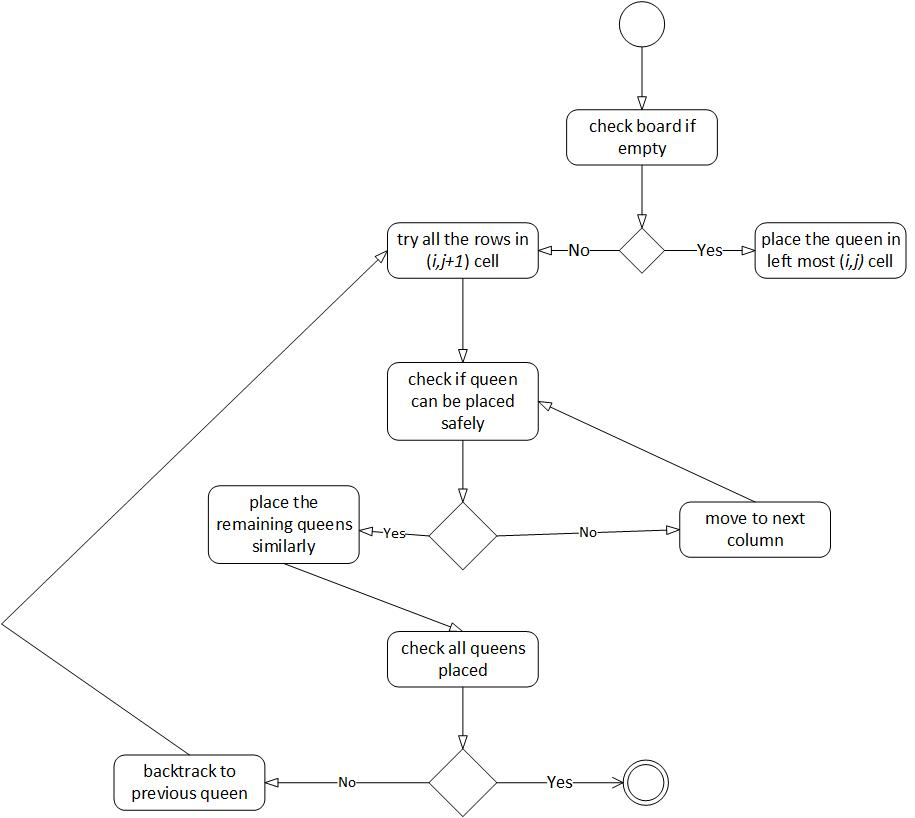
\includegraphics[scale=0.5]{activity8queen.jpg}
	\end{figure}
	
\bigskip
\bigskip
\bigskip
\bigskip



\end{itemize}

\newpage
\noindent {\bfseries Mathematical Model:}

{\ttfamily
\textrm{Consider a set S consisting of all the elements related to a program.The mathematical model is given as below,}}

\subsubsection[S= \{s, e, X, Y, Fme, DD, NDD, Mem shared\}]{\rmfamily S= \{s, e, X, Y, Fme, DD, NDD, Mem shared\}}
\subsubsection[Where,]{\rmfamily Where,}
\subsubsection[s = Initial State]{\rmfamily s = Initial State}
\subsubsection[e = End State]{\rmfamily e = End State}
\subsubsection[X = Input. Here it is map size, start point]{\rmfamily X = Input. Here it is map size, start
point}
\subsubsection[Y = Output. Here output is time required to generate route, actual route\ \ \ and map.]{\rmfamily Y =
Output. Here output is time required to generate route, actual route\ \ \ and map.}
\subsubsection[Fme = Algorithm/Function used in program.\ ]{\rmfamily Fme = Algorithm/Function used in program.\ }
\subsubsection[For e.g.\ placequeen() etc.]{\textmd{For e.g.}\ \textmd{placequeen() etc.}}
\subsubsection[DD=Deterministic Data]{\rmfamily DD=Deterministic Data}
\subsubsection[NDD=Non deterministic Data]{\rmfamily NDD=Non deterministic Data}
\subsubsection[Mem shared=Memory shared by processor.]{\rmfamily Mem shared=Memory shared by processor.}

\bigskip


\bigskip

{\bfseries
Algorithm:\ }


\bigskip

{\ttfamily
\textrm{\textbf{Backtracking Algorithm:\ }}}


\ \ \ \ \ \ \ \ \ The idea is to place queens one by one in different columns, starting from the leftmost column. When
we place a queen in a column, we check for clashes with already placed queens. In the current column, if we find a row
for which there is no clash, we mark this row and column as part of the solution. If we do not find such a row due to
clashes then we backtrack and return false.


\bigskip

{\bfseries
1.\ Start in the leftmost column}

{\bfseries
2.\ If all queens are placed return true}

{\bfseries
3.\ Try all rows in the current column. \ Do following for every tried row.}

{\bfseries
\ \ \ \ a.\ If the queen can be placed safely in this row then mark this [row, column] as part of the solution and
recursively check if placing queen here leads to a solution.}

{\bfseries
\ \ \ \ b.\ If placing queen in [row, column] leads to a solution then return true.}

{\bfseries
\ \ \ \ c.\ If placing queen doesn't lead to a solution then umark this [row, Column] (Backtrack) and go to step (a) to
try other rows.}

{\bfseries
4.\ If all rows have been tried and nothing worked, return false to trigger backtracking.}


\bigskip



\bigskip


\bigskip

\noindent \textbf{Testing:}
\begin{itemize}
\item \textbf{Positive Testing:}\\
Positive Testing is testing process where the system validated against the valid input data. In this testing tester always check for only valid set of values and check if a application behaves as expected with its expected inputs. The main intention of this testing is to check whether software application not showing error when not supposed to and showing error when supposed to.

The system will show the appropriate output when it is tested against correct mathematical values. For example, for trigonometric functions, the system will show appropriate output in floating point numbers. Also for basic mathematical operations like addition, subtraction, it will show appropriate output.\\
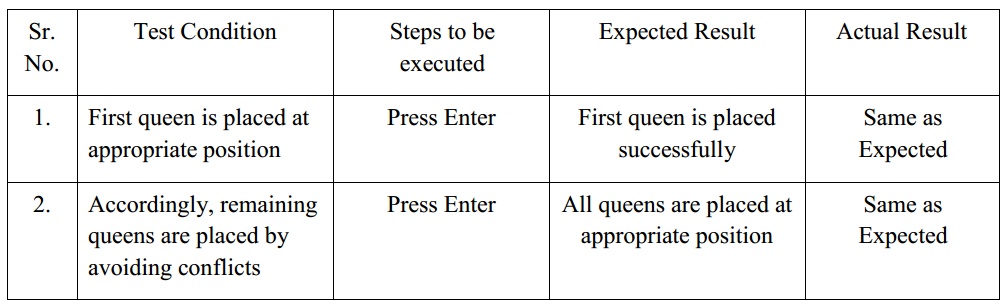
\includegraphics[width=\textwidth]{queen_positive}


\item \textbf{Negative Testing:}\\
Negative Testing is testing process where the system validated against the invalid input data. A negative test checks if a application behaves as expected with its negative inputs. The main intention of this testing is to check whether software application not showing error when supposed to and showing error when not supposed to.

While performing the negative testing, the system will show incorrect output while performing the basic arithmetic operations if the user enters only a single number and performs addition without entering the second number. The system will give an error when the user attempts a divide by zero operation.\\
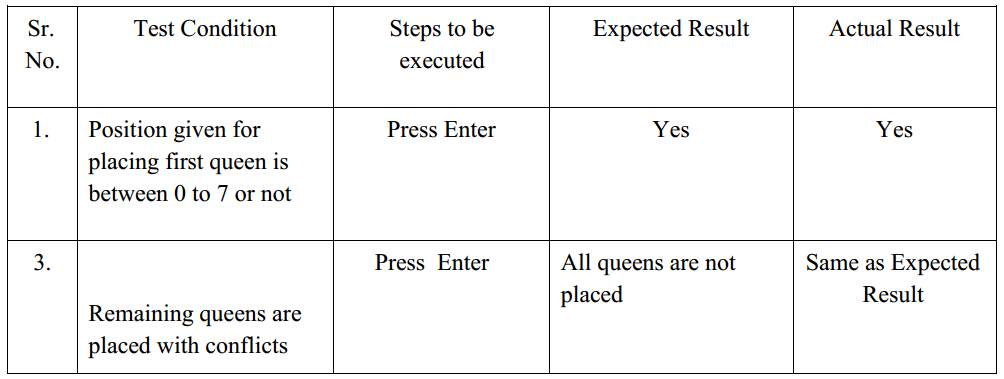
\includegraphics[width=\textwidth]{queen_negative}

\end{itemize}


\begin{itemize}
\newpage
\item \textbf{Test cases using black box and white box testing:}
\begin{enumerate}
\item Test case:Part 1
\end{enumerate}
\begin{figure}[h!]
		\centering
		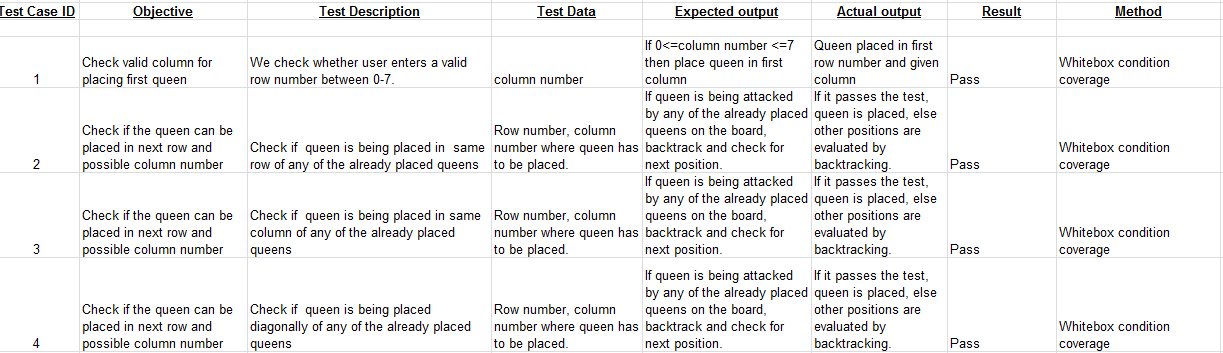
\includegraphics[scale=0.5]{queentest1.png}
	\end{figure}
    
\begin{enumerate}
\item Test case: Part 2
\end{enumerate}

\begin{figure}[h!]
		\centering
		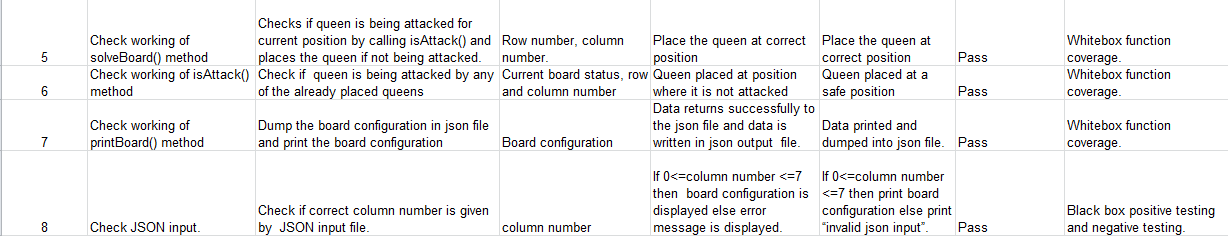
\includegraphics[scale=0.5]{queentest2.png}
	\end{figure}
\end{itemize}
\bigskip

{\sffamily
\textrm{\textbf{\textcolor{black}{CONCLUSION:\ }}}}\\

{\sffamily
\textrm{\textbf{\textcolor{black}{\ \ }}}\textrm{\textcolor{black}{Hence we\ implemented}}\textrm{\ 8
queen\ problem\ using\ backtracking in python and studied different design and testing methods.}}

\begin{center}
\begin{tabular}
{|c|c|c|c|c|}\hline
{\bf Roll No.}		&{\bf Name of Student}	&{\bf Date of Performance}  				&{\bf Date of Submission}	&{\bf Sign.}  \\    \hline
{302}	&	{Abhinav Bakshi}& 	{21/03/16}	&  {30/03/16} \\ \hline
\end{tabular}\\ 
\end{center}	

\begin{figure}[htb!]
	\centering
	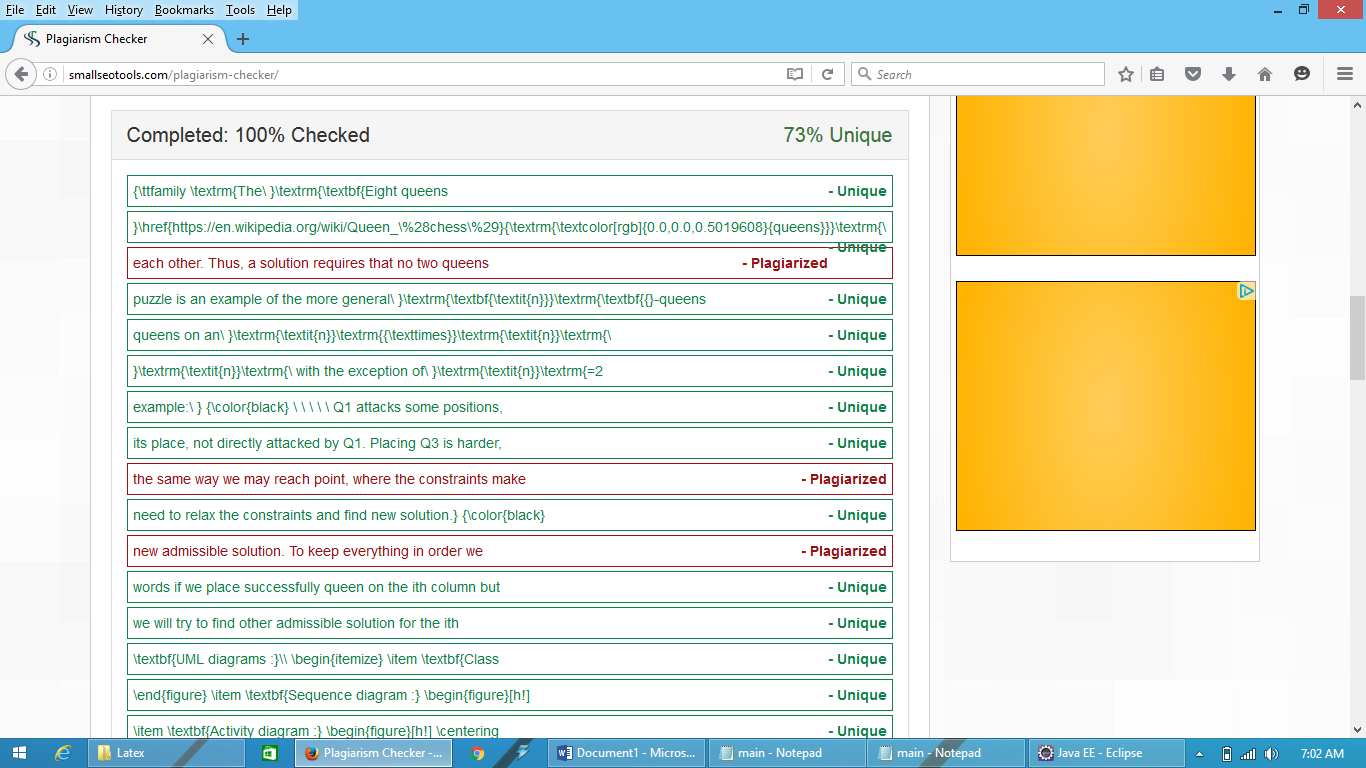
\includegraphics[scale = 0.75]{b6_8queen.png}
	\caption{Plagiarism Report }
	\label{Plagiarism Report}
\end{figure}


\end{document}
